\label{chapter-analysis}

In this chapter, I analyse the data that have been extracted by {\tt eth2dgraph}. Each section describes an independent analysis.

All the results refer to data from block $0$ to block $17,265,420$ of the Ethereum {\tt mainnet}. It corresponds to the period of time between July 30 2015 to May 15 2023 (7 years, 9 months, and 15 days).

\section{General data overview}

This analysis is conducted to give a general overview of the data extracted. There are some interesting analysis results that help to understand the current state of the Ethereum chain. Here are some interesting points:

\begin{itemize}
    \item 60,016,663 smart contract deployments, of which 213,406 failed, were found with 59,429,189 unique addresses. 88\% of them (52,343,783) never emitted logs. 87\% of them (51,974,197) never received a single transaction. Just 5.78\% (3,435,332) of contracts' addresses both received at least one transaction and emitted at least one log. This shows that the vast majority of the deployed smart contracts are never actively used. \Cref{fig:contracts-by-usage} shows the distribution of smart contracts based on their active usage.
    
    \item There are 2.8B logs emitted. 10 smart contracts alone, reported in \cref{table:top-logs-emitters}, emitted the 24.25\% of all logs. Top 100 contracts emitted 38.83\% of the logs. Top 1,000 contracts emitted 57.53\% of the logs. 33,287 smart contracts (0.056\% of the total) emitted 90\% of the logs. Most of the activity on the chain is restricted to a relatively small group of smart contracts.
    
    \item Transactions are more evenly distributed compared to logs. There are 165,684,328 distinct EOAs that have sent transactions. Top 10 senders sent 6.96\% of all transactions. 90\% of transactions were sent by top 25\% addresses. 
    
    \item There are 286,391,265 distinct addresses that have received transactions. The top 10 receivers received 18.55\% of all the transactions, and there is just one receiver in the top 10 that is not a contract\footnote{It is an address of the Coinbase exchange {\tt 0xa090e606e30bd747d4e6245a1517ebe430f0057e}.}. 90\% of transactions were received by the top 57.85\% receivers.
    
    \item 61.92\% of transactions are sent to smart contracts. 0.25\% are sent to the null address {\tt 0x0}. The remaining 37.83\% are transactions from EOAs to other EOAs or unclaimed addresses.
    
    \item \cref{fig:deploy-history} shows the history of smart contracts deployments. The growth in deployments was exponential until the beginning of 2018. After an initial period in which there were more deployments done by users than by contracts, now the majority of smart contracts are deployed using the CREATE or CREATE2 opcodes. This confirms the trend observed by Kiffer et al.~\cite{ethereum-sc-topology}. They observed this phenomenon in data until 2018. The difference in deployments by users or by contracts has grown since then. Since 2019, the difference has been of at least one order of magnitude.
\end{itemize}

\begin{figure}[!ht]
    \centering
    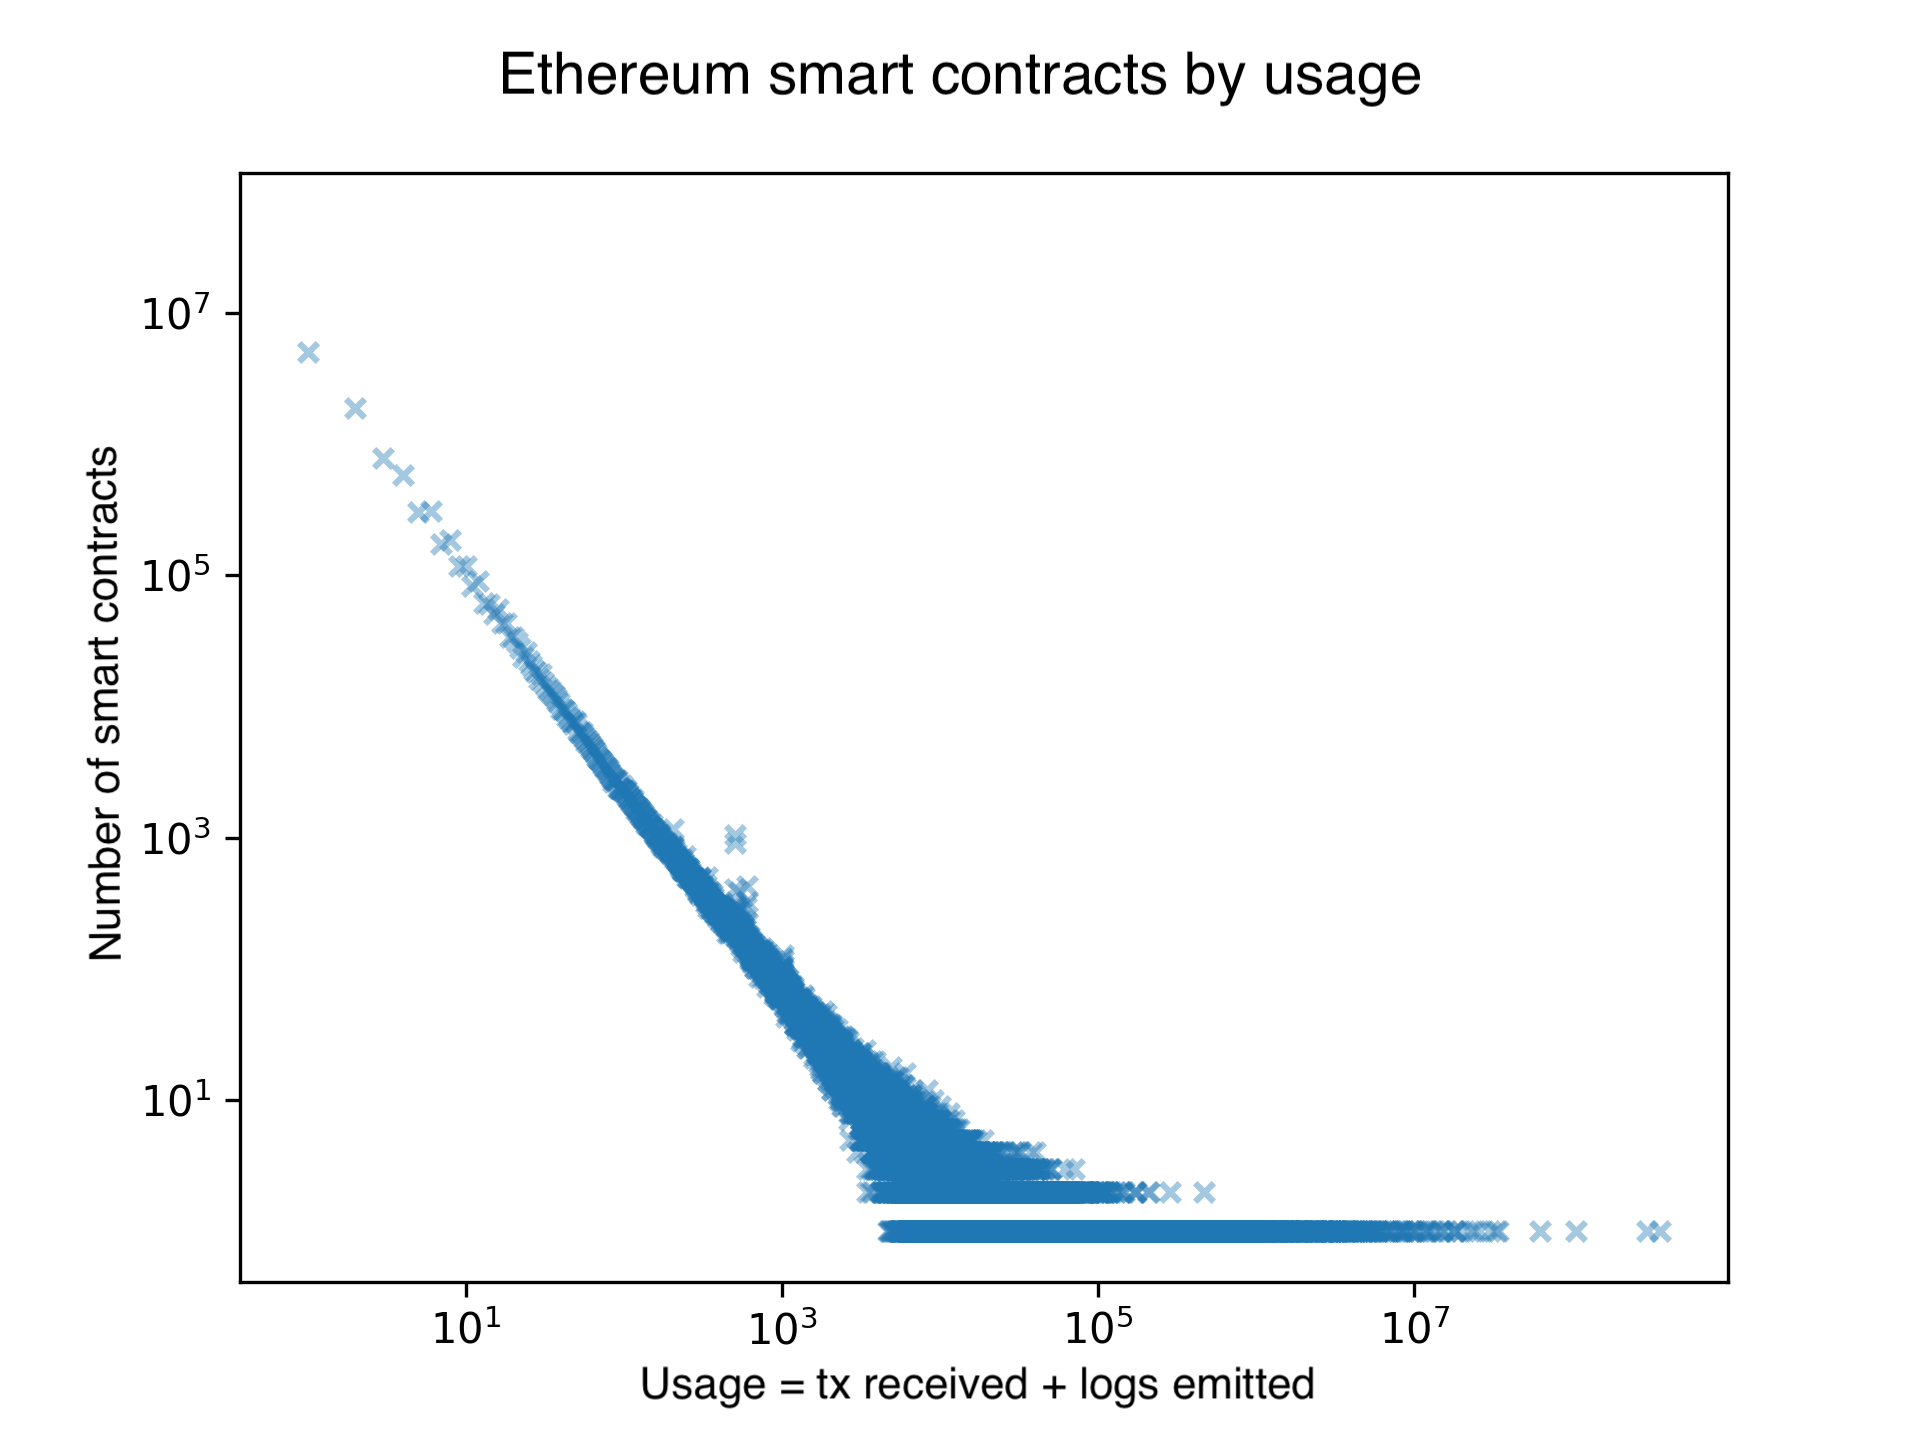
\includegraphics[width=1\textwidth]{Figures/analysis/contracts_by_usage.png}
    \caption{Ethereum smart contracts by usage, note the log scale on both axes.}
    \label{fig:contracts-by-usage}
\end{figure}

\begin{table}[!ht]
\centering
    \begin{threeparttable}
    \begin{tabular}{ c c c } 
    \toprule
    \textbf{Name of contract} & \textbf{Contract address} & \textbf{Logs emitted} \\
    \midrule
       Wrapped Ether & \small{0xc02aaa39b223fe8d0a0e5c4f27ead9083c756cc2} & 282,095,104  \\ [1.2ex]
       Tether USD  & \small{0xdac17f958d2ee523a2206206994597c13d831ec7} & 196,788,993  \\ [1.2ex]
       USD Coin & \small{0xa0b86991c6218b36c1d19d4a2e9eb0ce3606eb48} & 74,321,927  \\ [1.2ex]
       XEN & \small{0x06450dee7fd2fb8e39061434babcfc05599a6fb8} & 30,438,737  \\ [1.2ex]
       DAI Stablecoin& \small{0x6b175474e89094c44da98b954eedeac495271d0f} & 20,283,129  \\ [1.2ex]
       Seaport & \small{0x00000000006c3852cbef3e08e8df289169ede581} & 16,764,010  \\ [1.2ex]
       ChainLink Token & \small{0x514910771af9ca656af840dff83e8264ecf986ca} & 16,698,857  \\ [1.2ex]
       Wyvern Exchange & \small{0x7be8076f4ea4a4ad08075c2508e481d6c946d12b} & 15,735,740  \\ [1.2ex]
       SHIBA INU & \small{0x95ad61b0a150d79219dcf64e1e6cc01f0b64c4ce} & 12,607,046  \\ [1.2ex]
       Forsage & \small{0x5acc84a3e955bdd76467d3348077d003f00ffb97} & 12,323,018  \\ [1.2ex]  
    \bottomrule
    \end{tabular}
    \end{threeparttable}
    \caption{Top 10 smart contracts per logs emitted.}
    \label{table:top-logs-emitters}
\end{table}

\begin{figure}[!ht]
    \centering
    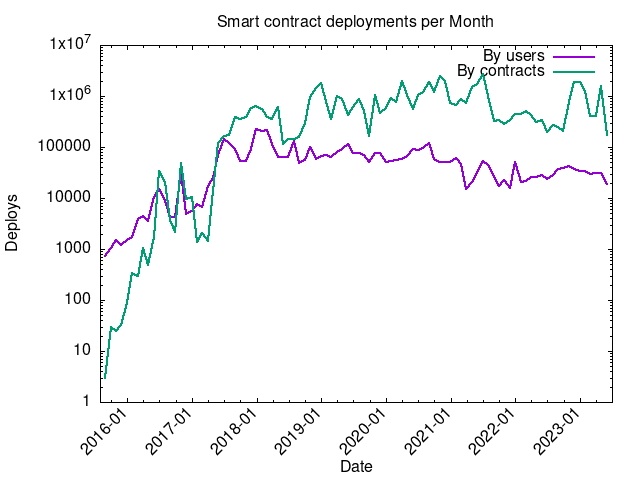
\includegraphics[width=1\textwidth]{Figures/analysis/deploys_per_month.png}
    \caption{Smart contract deployments over time grouped by month.}
    \label{fig:deploy-history}
\end{figure}

\newpage

\section{Skeleton clusters}

The skeleton of a smart contract is its deployed bytecode without the arguments of the PUSH opcodes and the eventual metadata appended at the end. \Cref{skeleton-section} describes this concept and explains how eth2dgraph extracts the skeletons from the Ethereum chain.

Out of the 60M smart contracts deployments in the history of Ethereum, just 467K distinct skeletons were found. This allows us to link smart contracts with each other based on skeleton equality. On average, each smart contract has 128 semantically identical siblings. 

The distribution of smart contracts by skeleton is not uniform. There are 361,546 skeletons (77.4\%) that correspond to a single deployed Ethereum smart contract. At the same time, there are skeletons that correspond to millions of smart contract deployments. The most frequently used skeleton matched 12.2M deployments and was related to gas tokens, as shown in \cref{most-deployed-skeletons}.

\subsection{Most deployed skeletons}
\label{most-deployed-skeletons}

I analyze the top 10 skeletons found on the Ethereum chain by a number of deployments. These 10 distinct skeletons correspond together to 44,389,576 smart contract deployments (73.96\% of the total).

\begin{itemize}

    \item The most used skeleton is related to gas reserves. It is the way gas tokens store gas when it is bought. The concept of the gas token is analyzed in \cref{gas-tokens}. This skeleton has a very simple bytecode that just allows a particular address, with a length of 14 bytes, to destroy the contract. The size of this skeleton is 21 bytes. It has been deployed 12,240,689 times.
    
    \item The second skeleton is the implementation of the ERC-1167\footnote{Specification of the ERC-1167 Minimal Proxy Contract: \url{https://eips.ethereum.org/EIPS/eip-1167}} logic. This bytecode consists of a minimal proxy that forwards all the calls it receives to a fixed hard-coded address. The size of this skeleton is of 45 bytes. It has been used 11,168,872 times.

    \item The third skeleton is again related to gas tokens. It is the same logic as the first described skeleton but with the allowed address of 15 bytes instead of 14. It has been used 6,829,142 times. Its size is 22 bytes.

    \item The fourth skeleton is simply the empty bytecode. It is valid in the Ethereum protocol to have empty smart contracts. 4,877,139 deployments with no bytecode were found.

    \item The fifth skeleton is again related to gas tokens. It is the same logic as the previous two but with the length of the allowed address of 20 bytes. 2,138,723 deployments matching this skeleton were found with a size of 27 bytes.

    \item The sixth skeleton represents 1,665,668 user wallets of the \textit{Bittrex} exchange\footnote{Bittrex is a crypto exchange platform: \url{https://global.bittrex.com/}.}. Each of these smart contracts is a controlled wallet. This means that each contract represents a user of the exchange, but the control over the Ethers and tokens remains under the company. The point of having these controlled wallets is to give users a unique address to send their tokens or Ethers. The size of this skeleton is of 502 bytes.

    \item The seventh skeleton has been used 1,549,146 times and represents an \textit{OwnableDelegateProxy}. It is a proxy contract, so it simply forwards the received calls to another contract that implements the actual logic, using {\tt delegatecall}. This specific type of proxy has two additional properties:
    \begin{itemize}
        \item \textit{Ownable}: it stores the address of the owner and allows it to modify the implementation address. The ownership can eventually be transferred.
        \item \textit{Upgradable}: it is possible to update the address of the implementation, changing where the proxy is forwarding the calls.
    \end{itemize}
    All the previous logic is implemented in a bytecode with a size of 1073 bytes.

    \item The eighth skeleton has been used 1,542,310 times and represents a \textit{forwarder contract}. This skeleton has two main public functions: \textit{flush()} and \textit{flushTokens(address)}. They are used to transfer ETH and tokens to a fixed parent address. The point of this kind of contract is to have multiple receive addresses for the same wallet. ETH transfers are automatically sent to the parent address, while tokens can be flushed with a transaction. Bitgo\footnote{Bitgo is a digital asset trust company: \url{https://www.bitgo.com/}} uses this contract in their implementation of the multi-signature wallet\footnote{Source code of the multi-signature wallet: \url{https://github.com/BitGo/eth-multisig-v2/tree/master}}. The size of this skeleton is of 785 bytes.

    \item The ninth skeleton is a proxy used for the Ambi Multisig wallet as found by di Angelo and Salzer~\cite{wallet-contracts}. It has been deployed 1,202,291, with a size of 88 bytes. 

    \item The tenth skeleton has been used 1,175,596 times and it is the exact same forwarding logic of the eighth skeleton. The few small differences are probably due to the compiler version or optimization level. Its size is 789 bytes.
    
\end{itemize}

I calculated cosine and interface similarity of the top 10 skeletons to find similarities between them and all the other skeletons. This formed seven clusters shown in \cref{table:top-skeletons-clusters}.

These 7 clusters describe 75.29\% of all the deployments that happened in the Ethereum blockchain. They can be grouped in just 4 distinct categories: \textit{gas token}, \textit{proxy}, \textit{wallet} and \textit{empty contract}.

\begin{table}[H]
\centering
    \begin{threeparttable}
    \begin{tabular}{ c c c c } 
    \toprule
    \textbf{\# Group} & \textbf{Distinct skeletons} & \textbf{Deployments} & \textbf{Category} \\
    \midrule  
    1 & 5 & 21,787,384 & Gas token \\ [1.2ex]
    2 & 6 & 11,169,089 & Proxy \\ [1.2ex]
    3 & 1 & 4,877,139 & Empty contract \\ [1.2ex]
    4 & 31 & 2,732,644 & Wallet \\ [1.2ex]
    5 & 5 & 1,863,898 & Wallet \\ [1.2ex]
    6 & 20 & 1,55,2654 & Proxy \\ [1.2ex]
    7 & 3 & 1,202,787 & Wallet \\ [1.2ex]
    \bottomrule
    \end{tabular}
    \end{threeparttable}
    \caption{Clusters formed by grouping top 10 skeletons with their similars.}
    \label{table:top-skeletons-clusters}
\end{table}

\subsection{New skeletons over time}

An interesting metric to observe is when the skeletons were first seen on the blockchain. This is a different indicator to the one shown in \cref{fig:deploy-history}, since it just shows when semantically new smart contracts are deployed, avoiding all the replicas.

\Cref{fig:skeletons-deploy} shows, for each month, the number of new skeletons found on the Ethereum chain. While the number of monthly deployments has not increased since 2021, the number of new monthly skeletons has kept increasing. This is also visible in \cref{fig:skeletons-ratio}, especially in the year 2022 in which the ratio between deployments and new skeletons was low compared to the past. From this data, it appears that code reuse is dropping. 

\begin{figure}[H]
    \centering
    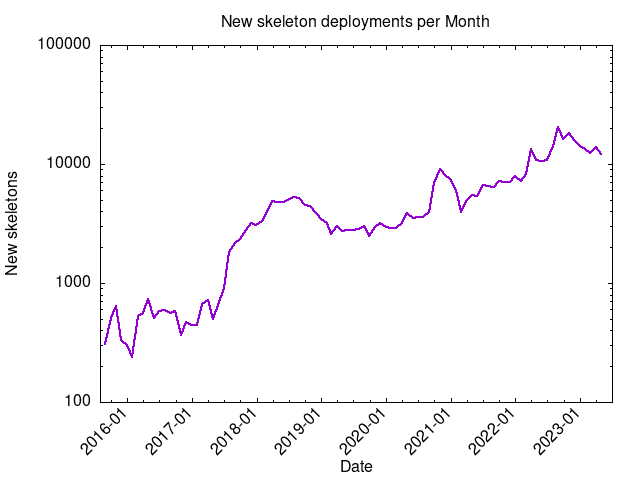
\includegraphics[width=0.9\textwidth]{Figures/analysis/skeletons_per_month.png}
    \caption{Deployments of new skeletons over time, grouped by month}
    \label{fig:skeletons-deploy}
\end{figure}

\begin{figure}[H]
    \centering
    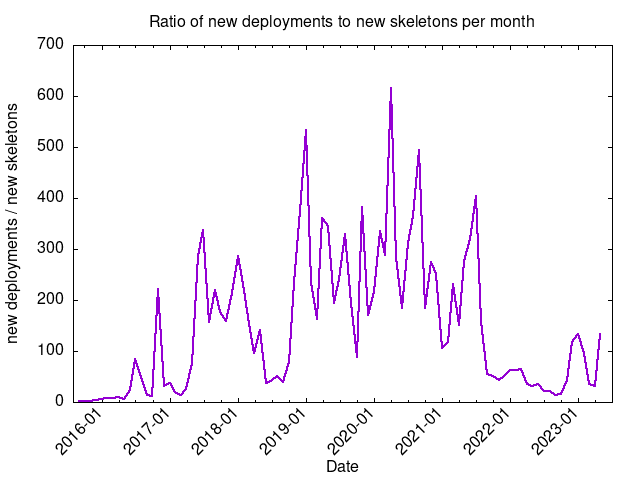
\includegraphics[width=0.9\textwidth]{Figures/analysis/ratio_per_month.png}
    \caption{Ratio of deployments to new skeletons over time, grouped by month. High values imply more duplicates deployed.}
    \label{fig:skeletons-ratio}
\end{figure}


\newpage

\section{Metamorphic contracts}

Smart Contracts are commonly thought to be immutable: once deployed on the Ethereum blockchain their code can not be changed. This was true until the introduction of the {\tt CREATE2} opcode in EIP-1014, included in the Constantinople Upgrade. This new opcode gives developers more control over the deployment address of the contracts created. 

With the {\tt CREATE} opcode, the new address is calculated as

\[a=keccak256(RLP(d,n_d))[12:] \]

in which $d$ denotes the \textit{deployer} address and $n_d$ the deployer \textit{nonce}. The nonce is updated by the protocol after every deployment. This prevents the possibility of deploying twice at the same address.

With {\tt CREATE2}, the newly created address is computed as

\[a=keccak256({\tt 0xff}\,||\,d\,||\,s\,||\,keccak256(c))[12:]\]

where {\tt 0xff} is a constant byte, $s$ is a salt picked by the deployer and c is the initialization code of the contract. The developer invoking {\tt CREATE2} has full control over all the variables, so it is easy to predict and manipulate the new address. The address to which the contract is deployed must be empty, this means that no contracts were ever deployed there or they were all previously destroyed.

With {\tt CREATE2} it is possible to deploy a smart contract to a certain address $a$, then destroy it and re-deploy it again with the same bytecode at the same address $a$. This event is called \textit{resurrection} by Fröwis and Böhme~\cite{create2-metamorphic}. 

Since the initialisation code of a contract can read the blockchain state, it is possible to use it in a way such that the same initialisation code, run multiple times, results in different deployed bytecodes. An easy way of doing so is by instructing it to ask for a third smart contract for the code to deploy. This third contract can change the code it gives back from time to time. This is one way of deploying different bytecodes at the same address, creating a \textit{metamorphic} smart contract. \cref{lst:meta-1,lst:meta-2} give an example of this pattern with pseudo code.

\begin{lstlisting}[label={lst:meta-1},caption={Pseudo initialization code that gets the code to deploy from another contract.}]
third_contract = address("0xab12...5134")
return third_contract.get_code()
\end{lstlisting}

\begin{lstlisting}[label={lst:meta-2},caption={Pseudo code of a contract that gives back the code to be deployed.}]
bytes code_to_deploy;

function setCode(bytes calldata _data) public {
    code_to_deploy = _data;
}
function getCode() public returns (bytes memory) {
    return code_to_deploy;
}
\end{lstlisting}

Another more complicated way to replace the deployed code of a contract is by combining {\tt CREATE} and {\tt CREATE2} together. {\tt CREATE2} is used to reset the nonce used in {\tt CREATE}. This can be done with the following steps:

\begin{enumerate}
    \item A deployer contract $D$ creates a \textit{factory} contract, here called $F$, at address $A_{f}$ using {\tt CREATE2}. $A_{f}$ is computed as $keccak256({\tt 0xff}\,||\,A_D\,||\,s\,||\,keccak256(c))[12:]$, in which $s$ is any random salt and $c$ is the initialization code of $F$.  

    \item Through $F$, a new contract $C_1$ is created using the {\tt CREATE} opcode at address $A_{c1}$. $A_{c1}$ will be calculated as $keccak256(RLP(A_f,n_d))[12:]$, in which $n_d$, the nonce, is zero.

    \item The factory $F$ is destroyed with {\tt SELFDESTRUCT} and redeployed again by $D$ at the same address $A_f$ and with the same code. This is achieved using {\tt CREATE2} with the same parameters. This step is needed to reset the nonce of $F$.

    \item The contract $C_1$ is destroyed with {\tt SELFDESTRUCT}.

    \item Now, $F$ can deploy a new contract with arbitrary code using {\tt CREATE}. The newly created contract will have the same address $A_{c1}$, since it is calculated as $keccak256(RLP(A_f,n_d))[12:]$ with $n_d$ equals to zero, as in step 2. 
    
\end{enumerate}

\subsection{Overview of metamorphic contracts usage}

Fröwis and Böhme~\cite{create2-metamorphic} analyzed metamorphic contracts until July 2021. They found 41 accounts that received deployments with different bytecodes. From a manual analysis, they concluded that this phenomena was used by just a few experienced users. They did not find any malicious use of this pattern. Most of the cases were about smart contracts related to the front-running infrastructure.

I here analyze the usage of this pattern in the data until May 15 2023, almost two years of data after the analysis conducted by Fröwis and Böhme.

A total of 267,461 accounts received multiple deployments of the \textbf{same} bytecode, these are the resurrected accounts. For the metamorphic pattern, there are 524 distinct accounts that have mutated bytecode over time. Out of these 524, 295 have probably used the pattern with just {\tt CREATE2}, since all the initialization codes were identical. While the remaining 229 accounts probably used the pattern combining {\tt CREATE} and {\tt CREATE2} since the deployments used different initialization codes. In total, these 524 accounts recorded 1,774 deployments and received 8,687,083 transactions. A CSV dump with many information related to metamorphic contracts has been published online at this address: \url{https://gist.github.com/davideaimar/e115098af481b16d6755b2e5acc04309}.

\begin{figure}
    \centering
    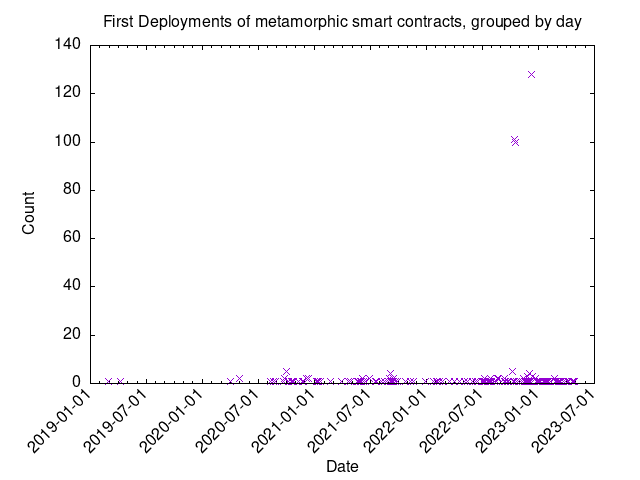
\includegraphics[width=0.9\textwidth]{Figures/analysis/metamorphic-first_deploys_outliers.png}
    \caption{First deployments of the metamorphic smart contracts.}
    \label{fig:meta-deploys-1}
\end{figure}

\begin{figure}
    \centering
    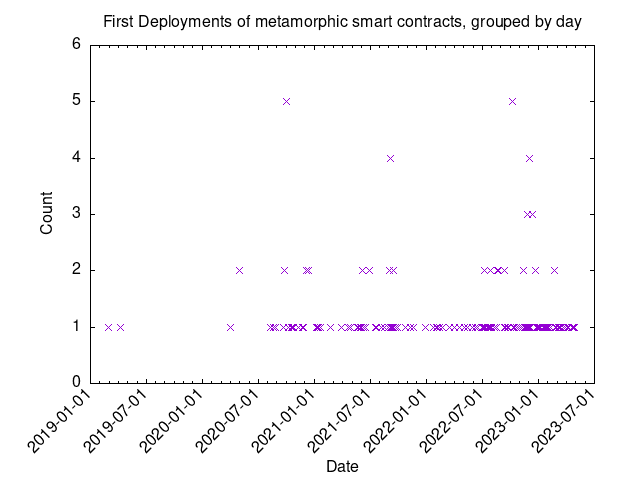
\includegraphics[width=0.9\textwidth]{Figures/analysis/metamorphic-first_deploys_no_outliers.png}
    \caption{First deployments of the metamorphic smart contracts without the three outliers.}
    \label{fig:meta-deploys-2}
\end{figure}

\begin{figure}
    \centering
    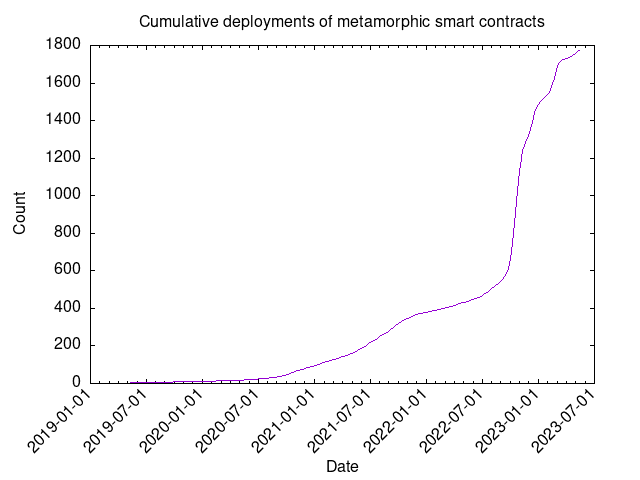
\includegraphics[width=0.9\textwidth]{Figures/analysis/metamorphic-all_deployments.png}
    \caption{Cumulative sum of all the metamorphic deployments.}
    \label{fig:meta-deploys-all}
\end{figure}

\Cref{fig:meta-deploys-1,fig:meta-deploys-2} show the first appearance of metamorphic contracts over time.
\Cref{fig:meta-deploys-1} shows all the data, while \cref{fig:meta-deploys-2} filter out three outliers. These three outliers are three days in which there were more than 100 first appearances of metamorphic smart contracts. These contracts are clearly correlated with each other. 

The cause these outliers were just two addresses\footnote{{\tt 0x3c3e8ab1e3327f24c917cd28789c9464adcf8198} and \\{\tt 0x6b25909c6141daf60ddf7c0700cedce07a9493d7} with respectively 596 and 256 metamorphic deployments.} that performed 852 deployments to metamorphic smart contracts in just three days. One of the addresses is used for MEV\footnote{MEV refers to multiple practices to maximize the extractable value from the block. It includes frontrunning, arbitrage and liquidations.} activity, while the other deployed metamorphic contracts that were all used to mint the XEN\footnote{XEN is an ERC-20 token available at \url{https://etherscan.io/token/0x06450dEe7FD2Fb8E39061434BAbCFC05599a6Fb8}} token.

\Cref{fig:meta-deploys-all} reports the cumulative sum of deployments to the 524 metamorphic smart contracts. In general, the usage of the metamorphic pattern has increased in the last period, especially since 2022.

As found by Fröwis and Böhme, many metamorphic contracts use \textit{vanity addresses}. These addresses have the peculiarity of having at least 7 leading zeros, meaning that they are smaller than the typical 20 bytes addresses. They are used to save on gas fees since it is less data that has to be stored on the blockchain. Out of the 524 metamorphic smart contracts found, 74 have a vanity address.

Understanding the purpose of metamorphic smart contracts is not easy. All the deployments do not have verified source code. Most of them have low-level bytecode with no decompiled functions (1660 out of 1781 deployments). 

I manually analyzed the top 110 metamorphic contracts by number of transactions received. I tried to understand their usage and I was able to flag the type of 98 contracts. 12 contracts were unclear what they were used for. Out of the 98 flagged contracts, 93 (94.89\%) contracts were found to be associated with MEV activity. This means that they were flagged as MEV by Etherscan or by Eigenphi\footnote{Eigenphi is a platform that collects and analyse blockchain data related to MEV activity. It is available at \url{https://eigenphi.io/}.}. The remaining 5 contracts were all used to mint the XEN token. 

This confirms the trend observed by Fröwis and Böhme, the metamorphic smart contracts are still restricted and used by a small number of users. Most of the metamorphic contracts that are effectively used for, or related to MEV activity. In many cases, the usage of this pattern is probably done for reusing vanity addresses, since they are hard to find and can have an impact on the MEV revenues.

\subsection{Similarity between metamorphic deployments}

To understand how much the code changes in between deployments of metamorphic contracts, I computed the cosine similarity between sequential deployments. For example, if a contract has received 3 deployments, I computed the similarity between the first and the second bytecodes and then between the second and the third bytecodes. The calculation of the similarity has been done as described in \cref{similarity-calculation}.

\begin{figure}
    \centering
    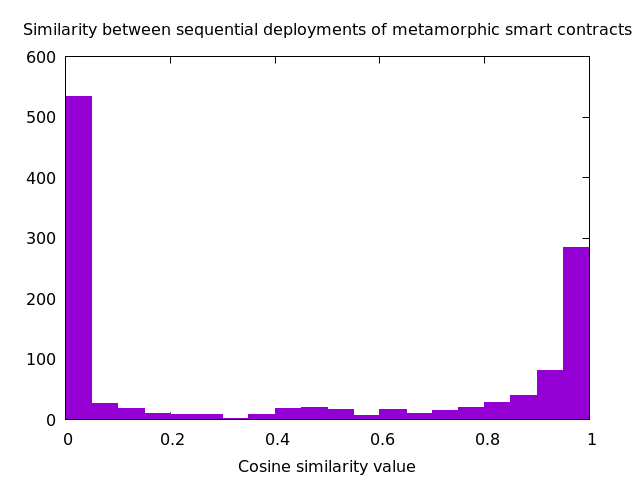
\includegraphics[width=0.9\textwidth]{Figures/analysis/metamorphic-similarities.png}
    \caption{Similarity values of all metamorphic deployments.}
    \label{fig:metamorphic-similarities}
\end{figure}
\begin{figure}
    \centering
    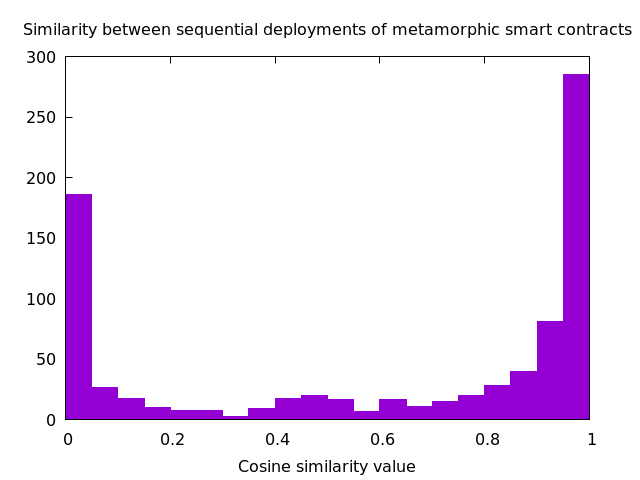
\includegraphics[width=0.9\textwidth]{Figures/analysis/metamorphic-similarities-no-pattern.png}
    \caption{Similarity values of metamorphic deployments excluding a pattern that occurred identically multiple times.}
    \label{fig:metamorphic-similarities-no-pattern}
\end{figure}

The resulting values are plotted in~\cref{fig:metamorphic-similarities}. A considerable amount of deployments completely changed the bytecode, with a similarity value of zero. Inspecting these bytecodes, I observed that most of these deployments were identical and followed a single pattern: 

\begin{itemize}
    \item The first and the second deployments were empty bytecodes.
    \item The third deployment was an implementation of the ERC-1167 minimal proxy contract.
\end{itemize}

All of the deployments that followed this pattern were done by the same address and were used to mint XEN tokens.

Excluding these deployments from the visualization showed that in the majority of cases the new bytecode is very similar to the one that is replaced. It is visible in~\cref{fig:metamorphic-similarities-no-pattern}.


\newpage

\section{Gas tokens}
\label{gas-tokens}

The aim of this analysis is to study the impact of the \textit{GasToken} pattern on Ethereum.

GasToken is a pattern that was heavily used on the Ethereum blockchain to save on gas fees. It exploited the concept of refund provided by the opcodes {\tt SELFDESTRUCT} and {\tt SSTORE}. 
I analyze and focus on the pattern that uses {\tt SELFDESTRUCT}. It works by creating and destroying basic smart contracts, used as gas reserves. 

This pattern caused the creation of many fuzzy contracts and state slots that increased the size of the Ethereum state. It was the main reason for the adoption of EIP-3529~\cite{eip-3529} on August 5th 2021. This EIP removed refunds for {\tt SELFDESTRUCT} and reduced {\tt SSTORE} refunds, effectively killing gas tokens. 

The following information explains how this pattern worked before EIP-3529. These two concepts are the fundamentals of this pattern: 

\begin{itemize}
    \item When a contract is deployed, the creator needs to pay $32000$ gas + $200$ gas for each non-zero byte stored.

    \item When a contract is destroyed, a refund of $24000$ gas is provided to the destroyer, after paying $700$ + $5000$ gas for calling {\tt CALL} + {\tt SELFDESTRUCT}. 
\end{itemize}

So the idea is that users deploy fuzzy contracts when gas is cheap and destroy them when gas is expensive. Gas from the refunds can cover up to 50\% of the gas used by the calling transaction that triggered the destructions, this is a limit introduced by the Ethereum protocol. 

To make this concept accessible, there are a few smart contracts that abstract the logic into simple tokens. For each token minted, there are many underlying smart contracts deployed. This token can easily be transferred between users. When the token is freed, the underlying smart contracts are destroyed and the owner of the token gets a discount on the gas of the transaction. The two most used tokens are CHI\footnote{Chi Gastoken on Etherscan: \url{https://etherscan.io/token/0x0000000000004946c0e9F43F4Dee607b0eF1fA1c}} and GST2\footnote{GST2 token on Etherscan: \url{https://etherscan.io/token/0x0000000000b3F879cb30FE243b4Dfee438691c04}}.

To be profitable, the price of the gas when tokens are bought must be at least half of the price of the gas when they are sold. 

Gas price has been historically very volatile, so the existence of this pattern makes sense.
\Cref{fig:gas-price} shows the historical fluctuation of gas prices.

\begin{figure}[!ht]
    \centering
    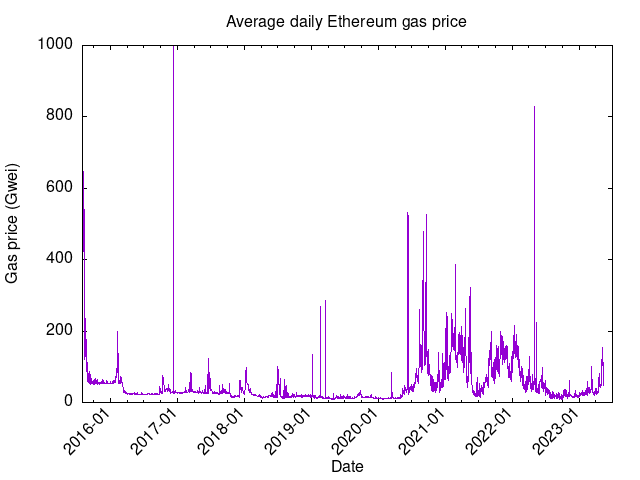
\includegraphics[width=0.9\textwidth]{Figures/analysis/gas-price.png}
    \caption{Average daily Ethereum gas price over time.}
    \label{fig:gas-price}
\end{figure}

\subsection{Identification of gas reserves}

I identified all the smart contracts ever deployed that were used as gas reserves. The logic of a gas reserve contract is basic. It simply allows one hard-coded address to destruct the contract. 
\Cref{lst:gas-token-code} shows the code that implements this logic, it is translated to the EVM bytecode reported in \cref{lst:gas-token-bytecode}

\begin{lstlisting}[caption={Pseudo code of the gas reserves.},label={lst:gas-token-code},captionpos=b,numbers=none]
if (msg.sender == GAS_TOKEN_ADDRESS) {
    SELFDESTRUCT(msg.sender);
}
\end{lstlisting}

\begin{lstlisting}[caption={EVM bytecode of the gas reserves.},label={lst:gas-token-bytecode},captionpos=b,numbers=none]
PUSH* <address of token contract>
CALLER
XOR
PC
JUMPI
CALLER
SELFDESTRUCT
\end{lstlisting}

The {\tt PUSH} opcode is represented as "{\tt *}" because there are different implementations of the gas reserve contract. Here it is possible to perform optimisations. The shortest the allowed address is and the fewer bytes are needed to be stored in the contract bytecode. This results in cheaper deployments and more efficiency of the pattern.

For example, the GST2 gastoken has this address: \\{\tt 0xb3f879cb30fe243b4dfee438691c04} that has just 15 bytes instead of the standard 20. The CHI gas token, a more recent and optimized alternative, uses\\ {\tt 0x4946c0e9f43f4dee607b0ef1fa1c} that is one less byte. Finding these short addresses is a very resource-intensive computation and requires trillions of iterations and hashes.

I identified all the gas reserves using the skeletons. There are five distinct skeletons that were used as gas reserves, with the only difference in the type of {\tt PUSH}. Some of the gas reserves were deployed multiple times at the same address. The data found is reported in \cref{table:gas-reserve-deployments}.

\begin{table}[H]
\centering
    \begin{threeparttable}
    \begin{tabular}{ c c c c } 
    \toprule
    \textbf{Skeleton} & \textbf{PUSH} & \textbf{Deployments} & \textbf{Distinct addresses} \\
    \midrule  
    \small{6d00...003318585733ff} & 14 & 12,216,500 & 12,188,707 \\ [1.2ex]
    \small{6e00...003318585733ff} & 15 & 6,809,029 & 6,765,219 \\ [1.2ex]
    \small{6f00...003318585733ff} & 16 & 568,116 & 525,202 \\ [1.2ex]
    \small{7000...003318585733ff} & 17 & 9,577 & 9,577 \\ [1.2ex]
    \small{7300...003318585733ff} & 20 & 2,138,608 & 2,138,608 \\ [1.2ex]
    \bottomrule
    \end{tabular}
    \end{threeparttable}
    \caption{Gas reserves found on Ethereum.}
    \label{table:gas-reserve-deployments}
\end{table}

A total of 21,741,830 successful gas reserve deployments were found, more than one third of all the deployments of Ethereum. 90.1\% of them have been destroyed, the remaining contracts are still alive. Users should pay gas to destroy them but without a reward is very unlikely that this will ever happen. There are 2,158,422 contracts that can potentially be stuck there forever since there is no incentive to remove them from the blockchain. The timeline of deployments and destructions is shown in \cref{fig:gastokens-timeline}. It is clearly visible how the London upgrade successfully killed this pattern.

\begin{figure}[!ht]
    \centering
    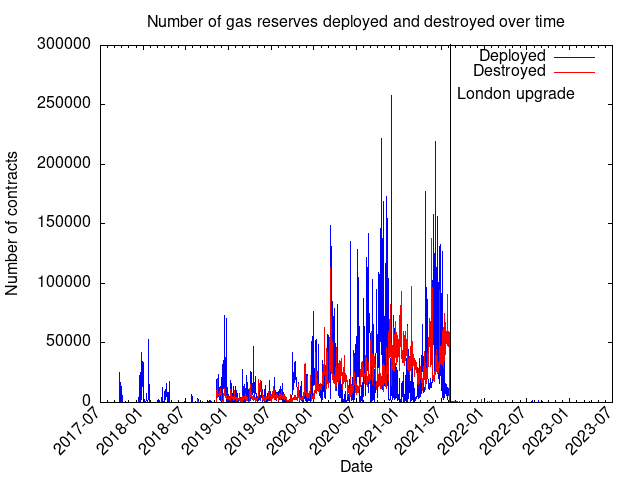
\includegraphics[width=0.9\textwidth]{Figures/analysis/gastokens-timeline.png}
    \caption{Deployments and destructions of gas reserves over time.}
    \label{fig:gastokens-timeline}
\end{figure}

\subsection{Quantification of eth saved}

I estimated the amount of Eth saved using the GasToken pattern. The calculation is performed on each gas reserve as:

\[eth_{saved}=eth_{refund}-eth_{mint}\]

\noindent where $eth_{refund}$ and $eth_{mint}$ are calculated as

\[eth_{refund} = gas_{refunded}*gas\_price_{refund\_ time}\]
\[eth_{mint}=gas_{mint}*gas\_price_{mint\_tine}\]

This is calculated on each gas reserve that was successfully deployed and then destroyed. This calculation is meant to give an order of magnitude of the amount saved.

These are the limitations and assumptions made for this calculation:

\begin{itemize}

    \item The gas spent for the small logic introduced by the token contracts that manage most of the gas reserves is not considered.
    
    \item Gas spent for the transactions that deployed the reserves is not considered. It highly depends on how many deployments were done in a single transaction. For example, doing 100 deployments in a single transaction (equivalent to minting 1 GST2 token) makes the gas of the transaction count for just 0.58\% of the deployment cost. I assume that all deployments were done in batches greater than 100 so the transaction cost is negligible.

    \item I assumed that all the destructions were done in such a way to not cover more than 50\% of the transaction gas with the refunds. Not doing so would mean wasting the refunded gas. 

    \item The gas prices used are the ones related to the blocks, obtained as the averages of the prices of gas in all the transactions. It is possible that many reserves were deployed by the miner themselves without paying for the gas.
    
\end{itemize}

The obtained value estimated a total saving of around 14K Eth, corresponding to 22,930,740 USD. The code used for this estimation is reported in \cref{lst:gas-calc}.

\begin{lstlisting}[language=Python,label={lst:gas-calc},caption={Code for computing the total Eth saved with the GasToken pattern.},captionpos=b]
# df contains all the gas reserves deployments 

# Type specifies wich PUSH was used (14, 15, ...)
# 24_000 is the refund
# 5_700 is the gas price for triggering SELFDESTRUCT + CALL
gas_refunded = 24_000 - 5_700 

# 32_000 is the cost of CREATE
# 200 is the cost for each byte stored
df['deploy_gas_used'] = 32_000 + 200 * ( 7 + df["type"] )
df['deploy_cost'] = df['deploy_price'] * df['deploy_gas_used']
df['destroy_reward'] = gas_refunded * df["destroy_price"]
df['profit'] = df['destroy_reward'] - df['deploy_cost']
saved = df['profit'].sum()
\end{lstlisting}

\newpage

\section{Most deployed functions and events}

Understanding what are the most commonly used functions and events gives a hint about what most smart contracts are doing.

I present in~\cref{table:top-functions,table:top-events} the most frequently deployed functions and events extracted using the Heimdall EVM decompiler. As explained in \cref{decompilation-section,cachine-section} the decompilation is performed on the deployed bytecode of the smart contracts, with a caching logic based on EVM skeletons. This means that two contracts sharing the same EVM skeleton received just one decompilation and the linked functions and events are the same. The numbers of this analysis depend directly on the accuracy of the decompiler.

\begin{table}[H]
\centering
    \begin{threeparttable}
    \begin{tabular}{ c c c } 
    \toprule
    \textbf{Function} & \textbf{Skeletons} & \textbf{Deployments}  \\
    \midrule
       \small{\tt sweep(address,uint256) -> bool} & 96 & 2,794,735\\ [1.2ex]
       \small{\tt flush()} & 182 & 2,775,935 \\ [1.2ex]
       \small{\tt flushTokens(address)} & 106 & 2,762,395 \\ [1.2ex]
       \small{\tt owner() -> address} & 57,643 & 2,226,240 \\ [1.2ex]
       \small{\tt tokenFallback(address,uint256,bytes)} & 68 & 1,897,675 \\ [1.2ex]
       \small{\tt implementation() -> address} & 1,472 & 1,688,820 \\ [1.2ex]
       \small{\tt proxyType() -> uint256} & 96 & 1,581,439 \\ [1.2ex]
       \small{\tt upgradeTo(address)} & 1,102 & 1,577,083 \\ [1.2ex]
       \small{\tt transferProxyOwnership(address)} & 177 & 1,556,545 \\ [1.2ex]
       \small{\tt proxyOwner() -> address} & 185 & 1,556,297 \\ [1.2ex]
       \small{\tt upgradeabilityOwner() -> address} & 127 & 1,554,012 \\ [1.2ex]
       \small{\tt upgradeToAndCall(address,bytes)} & 8 & 1,550,005 \\ [1.2ex]
       \small{\tt transferOwnership(address)} & 46,597 & 581,149 \\ [1.2ex]
       \small{\tt balanceOf(address) -> uint256} & 57,144 & 563,664 \\ [1.2ex]
       \small{\tt name() -> bytes memory} & 55,842 & 535,428 \\ [1.2ex]
       \small{\tt symbol() -> bytes memory} & 54,714 & 530,246 \\ [1.2ex]
       \small{\tt totalSupply() -> uint256} & 54,511 & 529,351 \\ [1.2ex]
       \small{\tt transfer(address,uint256)} & 46,024 & 526,022 \\ [1.2ex]
       \small{\tt approve(address,uint256) -> uint256} & 51,984 & 515,168 \\ [1.2ex]
       \small{\tt decimals() -> bool} & 44,682 & 503,589 \\ [1.2ex]
    \bottomrule
    \end{tabular}
    \end{threeparttable}
    \caption{Top 20 functions by number of deployments.}
    \label{table:top-functions}
\end{table}

\begin{table}[H]
\centering
    \begin{threeparttable}
    \begin{tabular}{ c c c } 
    \toprule
    \textbf{Event} & \textbf{Skeletons} & \textbf{Deployments}  \\
    \midrule
       \small{\tt TokensFlushed(address,uint256)} & 14 & 2,720,369\\ [1.2ex]
       \small{\tt Upgraded(address)} & 1,115 & 1,577,868\\ [1.2ex]
       \small{\tt ProxyOwnershipTransferred(address,address)} & 165 & 1,556,455\\ [1.2ex]
       \small{\tt OwnershipTransferred(address,address)} & 41,985 & 516,317\\ [1.2ex]
       \small{\tt Transfer(address,address,uint256)} & 47,380 & 494,780 \\ [1.2ex]
       \small{\tt Approval(address,address,uint256)} & 48,499 & 482,358 \\ [1.2ex]
       \small{\tt OwnerChanged(address)} & 133 & 430,676 \\ [1.2ex]
       \small{\tt DeedClosed()} & 4 & 430,173 \\ [1.2ex]
       \small{\tt SafeModeActivated(address)} & 51 & 231,379 \\ [1.2ex]
       \small{\tt TokenTransfer(address,address,uint256)} & 11 & 84,781 \\ [1.2ex]
       \small{\tt Transfer(address,uint256)} & 64 & 63,185 \\ [1.2ex]
       \small{\tt TokenReleased(address,uint256)} & 14 & 49,736 \\ [1.2ex]
       \small{\tt Burn(address,uint256)} & 3,136 & 37,404 \\ [1.2ex]
       \small{\tt OwnershipRenounced(address)} & 2,408 & 24,993 \\ [1.2ex]
       \small{\tt ApprovalForAll(address,address,bool)} & 10,063 & 22,451 \\ [1.2ex]
       \small{\tt AdminChanged(address,address)} & 520 & 20,353 \\ [1.2ex]
       \small{\tt LogSetOwner(address)} & 196 & 16,921 \\ [1.2ex]
       \small{\tt DelegateUpgraded(address,address,uint256)} & 2 & 14,076 \\ [1.2ex]
       \small{\tt DelegateRolledBack(address,address,uint256)} & 2 & 14,076 \\ [1.2ex]
    \bottomrule
    \end{tabular}
    \end{threeparttable}
    \caption{Top 20 events by number of deployments.}
    \label{table:top-events}
\end{table}

All the functions are related to proxy, wallet, or token contracts. For the events, it is the same situation. There is the event {\tt DeedClosed} that is related to ENS\footnote{ENS (Ethereum Name Service) is a decentralized name service \url{https://ens.domains/}.} and  {\tt DelegateUpgraded} and {\tt DelegateRolledBack} that are used for the Rocket Pool\footnote{Rocket Pool is a decentralized staking pool \url{https://rocketpool.net/}.} protocol, but both of these protocols are token-based.

\newpage

\section{Contracts metadata}

Smart contracts deployed using the Solidity compiler have the default option to include CBOR-encoded data at the end of the deployed bytecode. This piece of information includes:

\begin{itemize}
    \item The hash of the contract metadata. The metadata includes any kind of information related to the smart contract, such as the ABI, the documentation, the settings of the compiler, etc. It also includes the hash of the source code, so a change in the source code causes a change in the metadata that consequently changes its hash. This hash can be used as an address to store and retrieve the actual metadata and source code of the contract on a decentralized file system.
    \item The type of the hash ({\tt bzzr0}, {\tt bzzr1} or {\tt IPFS}).
    \item A flag stating if the compilation was done with experimental features of the compiler enabled.
    \item The version of the Solidity compiler used.
\end{itemize}

All of this data has been extracted by eth2dgraph with a regex as explained in \cref{skeleton-section}. Here is an overview of what has been extracted.

\subsection{Hash of metadata}

A total 17,491,909 deployments included the hash of the metadata in the bytecode stored on the blockchain. Out of these, 1,164,973 (6.66\%) used {\tt IPFS}, 15,636,747 (89.39\%) used {\tt bzzr0} and 690,189 (3.94\%) used {\tt bzzr1}. 

Analyzing the values of the hashes, there were just 770,719 distinct hashes found. This means that, on average, each smart contract compiled with the Solidity compiler gets deployed 22.7 times, another indicator of the high code reuse in the Ethereum blockchain. There are five occurrences in which the same metadata hash has been deployed more than 1M times, all of these deployments were done by just a few distinct addresses. On the other hand, there are 690,157 occurrences in which the hash was only used once.

\subsection{Experimental compilations}

The Solidity compiler allows to activate experimental features that are not already included by default in the decompiler. This can be done at the beginning of the code writing {\tt pragma experimental <feature-name>}. Inside the CBOR encoded data appended at the end of the generated bytecode there is a boolean stating whether any experimental feature was used or not.

Out of the 17,491,909 deployments that included the CBOR encoded data, 1,113,139 (6.36\%) had experimental features activated. These contracts with experimental features received a total of 5.8M transactions.

\subsection{Solc versions}

2,090,487 smart contracts included the version of the Solidity compiler in the CBOR-encoded data. The version is included just from Solidity v0.5.9 onward. There are 1,299 smart contracts that included fake Solidity versions (e.g. 100.67.137, 116.153.33, etc.) and were removed in this analysis. 32 deployments were found to use pre-releases of the compiler, in these cases Solidity appends the exact commit used. The total numbers of major versions found are reported in~\cref{table:solc-majors}.

\begin{table}[ht]
\centering
    \begin{threeparttable}
    \begin{tabular}{ c c } 
    \toprule
    \textbf{Major Solidity version} & \textbf{Number of deployments} \\
    \midrule
       0.5 & 925,506 \\ [1.2ex]
       0.6 & 287,552 \\ [1.2ex]
       0.7 & 215,924 \\ [1.2ex]
       0.8 & 660,206 \\ [1.2ex]
    \bottomrule
    \end{tabular}
    \end{threeparttable}
    \caption{Numbers of deployments found per major version of the Solidity compiler.}
    \label{table:solc-majors}
\end{table}

\Cref{fig:deploys-per-solidity-version} shows the distribution over time of the various major Solidity versions found. 
Generally, it is possible to observe how old compiler versions remain heavily used even after the release of multiple new versions.
The versions 0.6 and 0.7 almost never managed to have a higher amount of daily deployments than the 0.5 version.
The latest version, 0.8, managed to overtake the 0.5 after around one year since its release. Now it is the most used Solidity version.

\begin{figure}[ht]
    \centering
    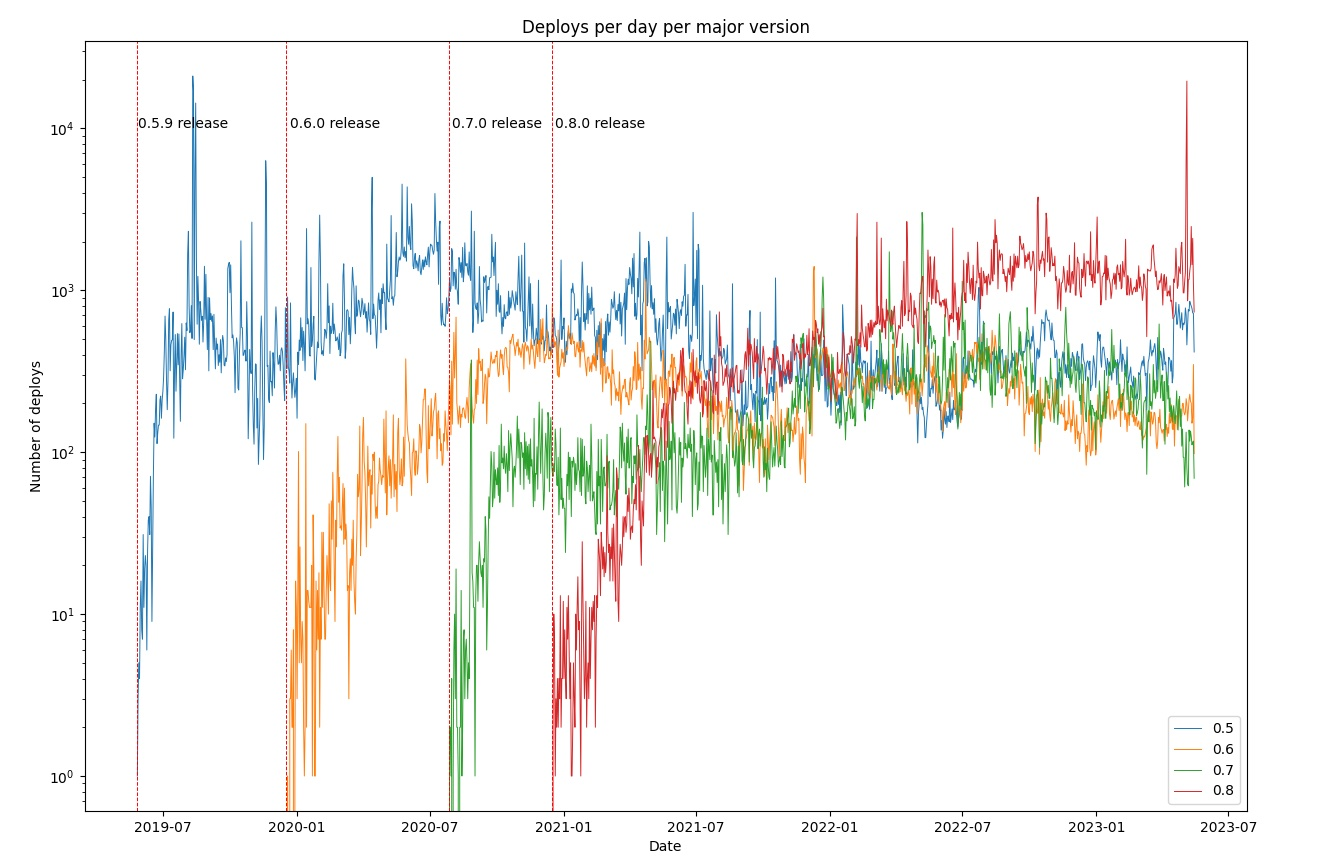
\includegraphics[width=0.95\textwidth]{Figures/analysis/deploys_per_day_per_major.jpg}
    \caption{Deployments over time divided by major Solidity compiler versions. Each data entry represents the daily amount of deployments found per version. Keep in mind the log scale.}
    \label{fig:deploys-per-solidity-version}
\end{figure}




